

\begin{figure}[!t]
	\centering
	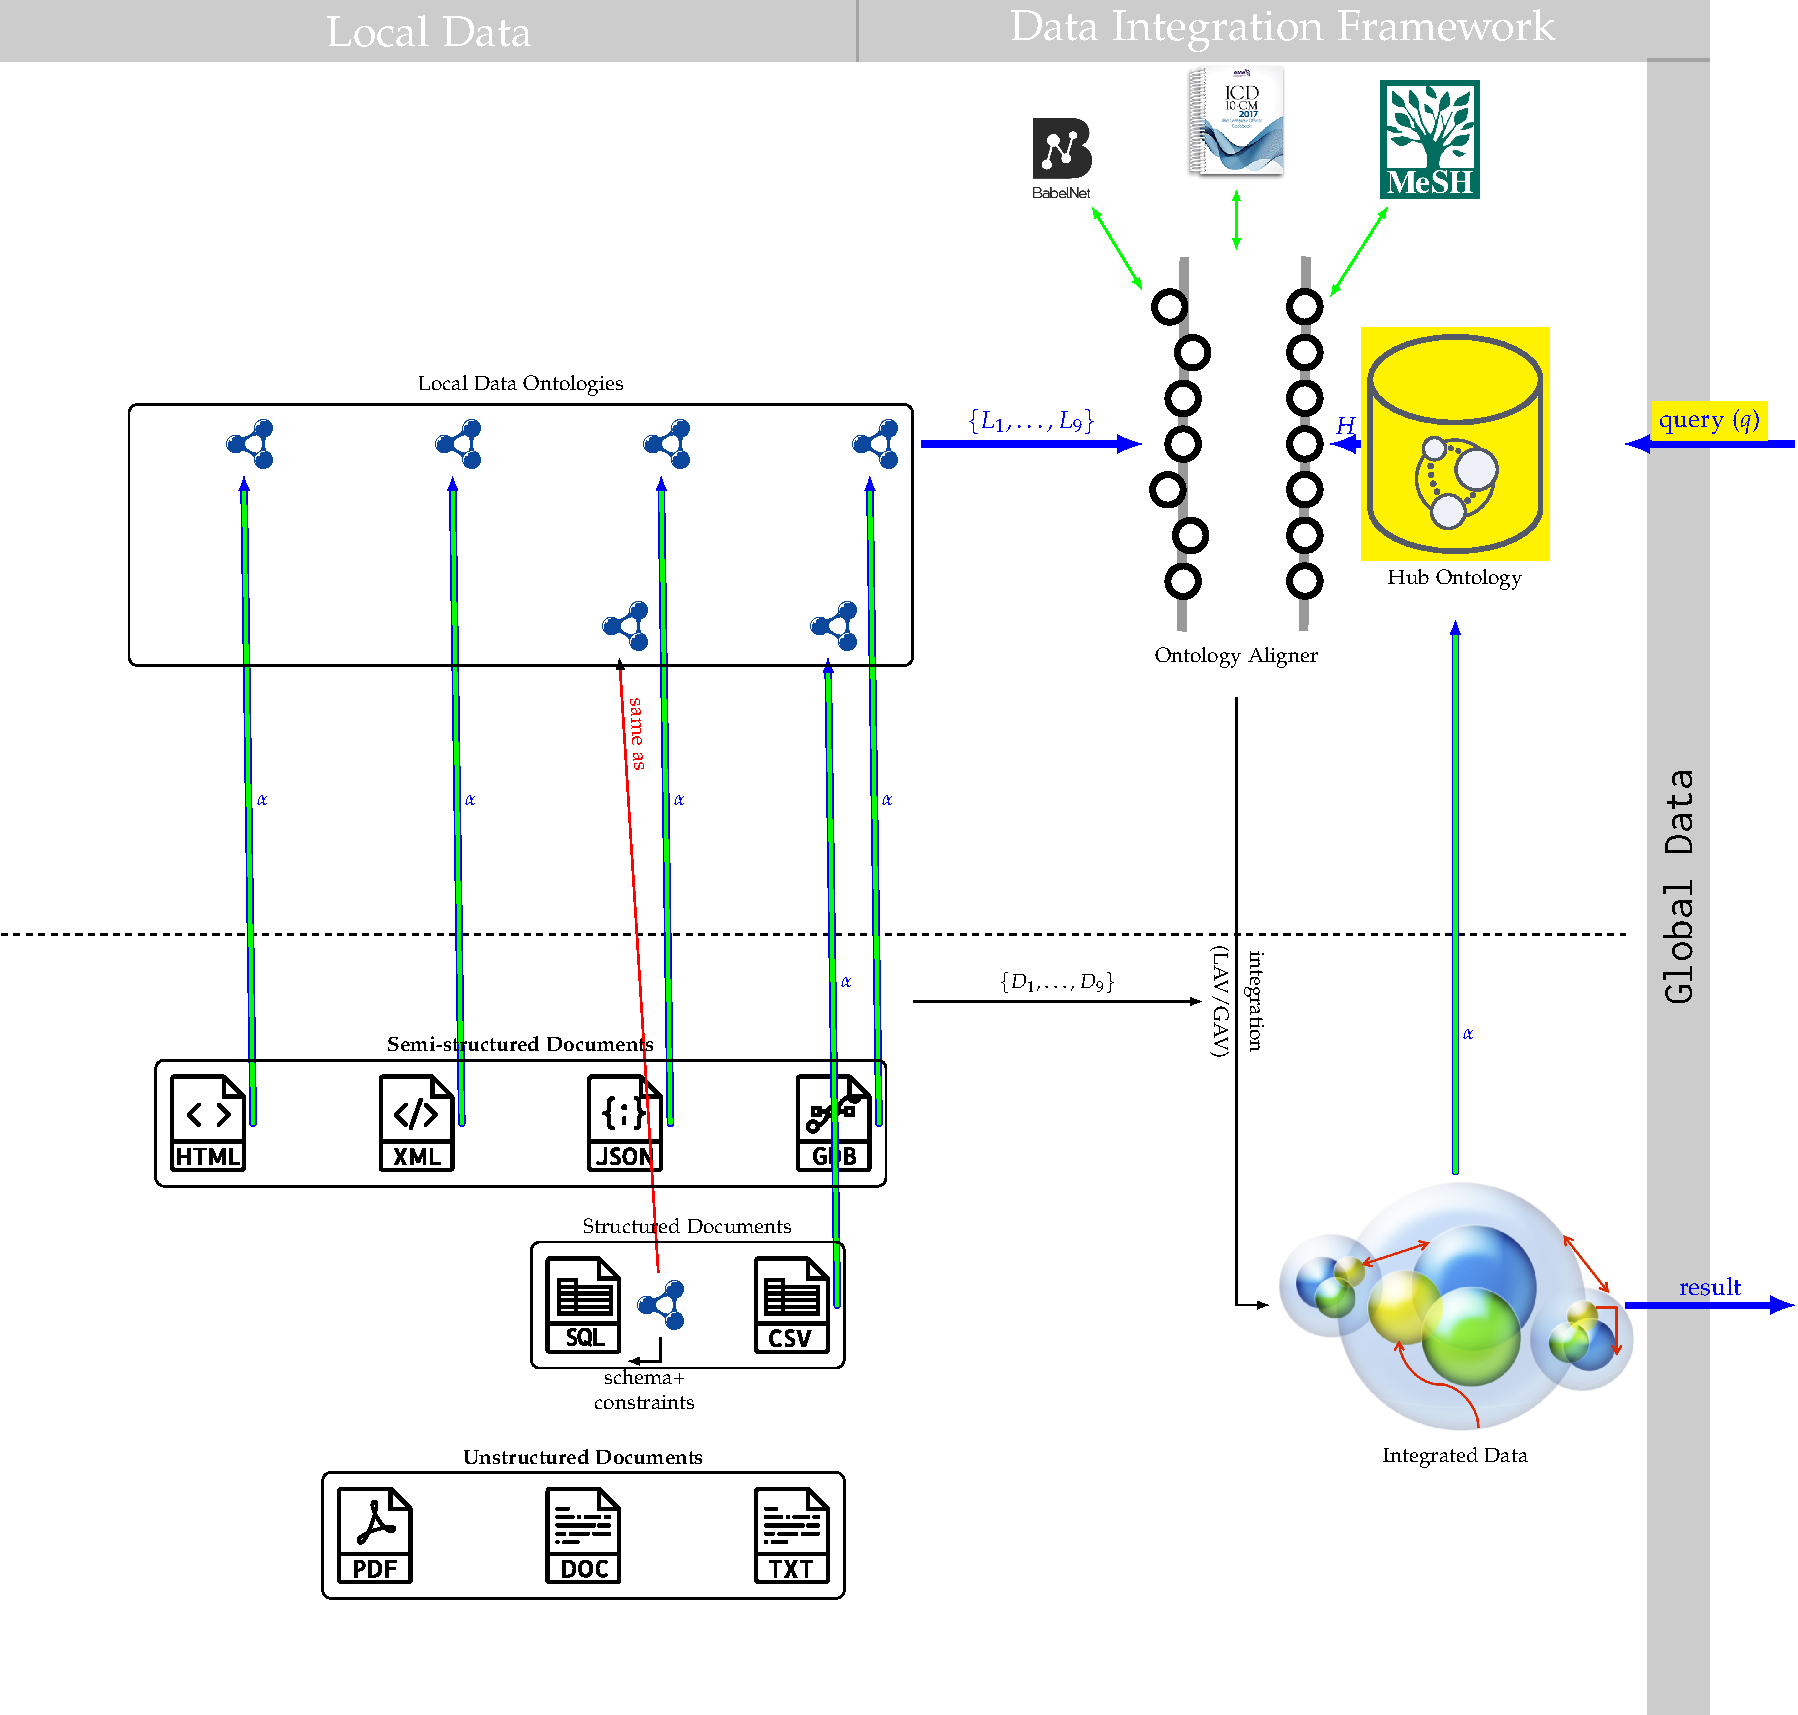
\includegraphics[width=\textwidth]{fig/01dataint/LAV}
	\caption{Representation of the data integration scenario of both the Local As a View and Global As a View approaches. Beside their definition, the only difference with this representation stands in the representation of the integrated data as either a materialized view of the local sources or as a temporarily query result. The components highlighted in yellow remark the parts that could be directly provided by the external user.}
	\label{fig:lavgav}
\end{figure}
\subsection{Query Rewriting}\label{subsec:queryrw}
In the last section we focused on performing data integration among different data sources and to reconcile them into one global representation in a data representation independent approach. At this point we should ask at  which stage we prefer to execute the query $q$, either on the still-to-be integrated data sources and then also after the data integration process (\textsc{Local As a View}, \cite{ManolescuFK01,Nadal0AVV17,SintSSF09}), or always at the end of such integration process (\textsc{Global As a View}, \cite{magnani04,Magnani06,Lu2006,BotoevaCCRX16}). These two approaches are interchangeable within the data integration task.

\begin{example}
By rephrasing the data integration approach in the latter subsection, Figure \ref{fig:lavgav} provides general data integration framework, where both such approaches could be used. The difference between the two approaches are hidded by the \textup{integration} arrow, that is going to be expanded and analyzed in the following definitions. Our local data either comes with an associated schema (e.g., the SQL dumps containing the constraints on the relational tables) or such schema should be extracted through ad hoc $\alpha$ functions, thus providing an ontology (represented in Figure with blue clique-3 graphs). All such local ontologies must be aligned to the main global hub ontology $H$, that is either directly provided by the user or obtained ``at runtime'' from the local ontologies by abstracting over each local schema \cite{BaaziziLCGS17}. If the data to be integrated contains general purpose concepts such as IBM Watson for Jeopardy \cite{IBMWatson}, then the Ontology Alignment process shall require intermediate general purpose ontologies for producing alignments, such as BabelNet for word relations and DBPedia for more complex and complete data. A more domain specific scenario, such as eHealth, requires more advanced and precise ontologies and taxonomies, such as MeSH and ICD-10 CM, such that the precision of the ontology alignment process can be increased.
\end{example}

We're now going to see that ontological alignments can be used within a more general data integration framework, that is   data representation dependent, and hence we have to introduce functions to   translate both data representation and   queries. The first class of functions is  represented by the class of \textbf{translation functions} $\ttransl_{D_1\to D_2}$, which convert the data representation in $D_1$ into $D_2$ in a purely syntactical way:
\begin{equation}
\label{eq:taufun}
\ttranslTHIS_{D_1\to D_2}\colon D_1\to D_2
\end{equation}

\begin{example}
The coding of a function allowing to transform a graph representation (Figure \vref{fig:inputbibex}) into a JSON one (e.g., Figure \vref{fig:jsongraphformat}) is straightforward, it is commonly used to export data from databases (dump) and does not require to use some specific knowledge concerning either the \textsc{Model} or the \textsc{Ontology} describing the data. Some data translation function will be provided in Section \vref{sec:tautonesting} for translating any possible data model into nested graphs.
\end{example}

The second operation is the query translation function\footnote{It is represented by the \texttt{qoppa} greek letter: $\qtransl,\qoppa$.} $\qtranslTHIS_{O_1,O_2}^A$\index{translation!query|see{$\qoppa$}} from a language $\langg_{O_1}$ to another language $\langg_{O_2}$ using the information of the alignment $\alignment(O_1,O_2)$ between the two ontologies for providing a translation of the query alongside its schema. More formally:
\[\qtransl\colon\forall O_1,O_2\in\mathcal{O}.\; A(O_1,O_2) \to \mathcal{L}_{O_1}\to \mathcal{L}_{O_2}\]
\[\qtransl_{O_1,O_2}^A=\qtransl (A(O_1,O_2))\quad s.t.\quad \qtransl_{O_1,O_2}^A\colon \mathcal{L}_{O_1}\to \mathcal{L}_{O_2}\]

The  \textsc{Global As a View} query rewriting approach, uses the alignments $A(\alpha(D_i),H)$  translating the local schema $\alpha(D_i)$ of database $D_i$ into a global view, thus performing the integration and the schema alignment within the same data representation of ${H}$. Using the aforementioned notation, such systems could be summarized with the composition of all the aforementioned functions as in the following definition:

\begin{definition}[Global As a View]\label{def:GAV}
	\index{data integration!global as a view|textbf}
Given a multisource data integration system $\Braket{H,\mathcal{I},\mathcal{O}}$ for a set of databases $\mathcal{D}=\Set{D_1,\dots,D_n}$ having their schemas in $\mathcal{O}$ ($\forall D_i\in\mathcal{D}. \alpha(D_i)\in\mathcal{O}$), a query $q$ could be run on heterogeneous data sources at the end of the data integration steps. First, we translate the data sources into a common representation ($\ttransl_{\alpha(D_i)\to H}(D_i)$). Given that a schema at the ontology level could even represent a query, such data is now aligned ($\qtransl_{\alpha(D_i),H}^A(\alpha(D_i))\big(\ttransl_{\alpha(D_i)\to H}(D_i)\big)$): now all the data are in the same representation, and hence they could be aggregated ($\nu_{\cong}(\dots)$) using a clustering algorithm among similar components \cite{ALIEH17}. Such aggregated data is then queried with $q$. As a result, we obtain the following expression:\index{$\nu$}

%% GAV(\Braket{H,\mathcal{I}},\mathcal{D},q) =
\[ q\left(\nu_\cong\left( \qtransl_{\alpha(D_1),H}^A(\alpha(D_1))\big(\ttransl_{\alpha(D_1)\to H}(D_1)\big), \dots, \qtransl_{\alpha(D_n),H}^A(\alpha(D_n))\big(\ttransl_{\alpha(D_1)\to H}(D_n)\big) \right)\right)\]
\end{definition}

This definition confirms the intuition expressed in \cite{Lenzerini02}, stating that GAV systems do not require the translation of the main query $q$ over the different data sources, but only on translating the local schemas into the global one. On the other hand, such systems could not optimize on-the-fly solutions where $q$ and $H$ are determined on the fly. Moreover, this is the traditional approach used in Data Warehouses, where data is extracted, transformed and processed to be compliant to the data warehouse schema expressed through an OLAP query \cite{Aligon201520}. Moreover, even in traditional data warehouses all the data must be converted into one final schema representation, that is here representeed by $H$ \cite{dwbook}.

With the second approach, called \textsc{Local As a View}, alignments are used to translate part of the query $q$ to be executed separately on the local sources. Then, the data is translated for the hub schema and integrated as in the previous phase, and then the remaining part of $q$ is run on the global representation.
	
\begin{definition}[Local As a View]
\index{data integration!local as a view|textbf}
Given a multisource data integration systems $\Braket{H,\mathcal{I},\mathcal{O}}$ for a set of databases $\mathcal{D}=\Set{D_1,\dots,D_n}$ having their schemas in $\mathcal{O}$, a query $q$ could be run on heterogeneous data sources by first performing a subquery of $q$ over the data that could be queried from $D_i$ accordingly to the alignment $A$ (hence, $q$ gets partially translated in $\qtransl_{H,\alpha(D_i)}^A(q)\big(D_i\big)$), then the data is necessarily transformed into the global representation $\ttransl_{\alpha(D_i)\to G}(\qtransl_{H,L_i}^A(q)\big(D_i\big))$. Later on, the data is integrated into a common data element, over which the remaining part of $q$, namely $q_{END}$, is processed to process the remaining part of the query requiring the combination of the pre-process data from the original sources. This process could be sketched as follows:

\[q_{END}\left(\nu_\cong\bigg(\ttransl_{\alpha(D_1)\to H}\Big(\qtransl_{H,\alpha(D_1)}^A(q)\big(D_1\big)\Big),\dots,\ttransl_{\alpha(D_n)\to H}\Big(\qtransl_{H,\alpha(D_n)}^A(q)\big(D_n\big)\Big)\bigg)\right)\]
\end{definition}


On the other hand, this approach is best suited for data that changes through time, and for which the ontology definition and the data representation could change. Despite the non-negligible cost of query rewriting, this solution provide a best solution when the final data schema could change at any possible query of the database. Nevertheless, this thesis is going to focus on the GAV approach, because it better separates the distinct operations that have to be performed in order to reach our final goal.